\chapter{Properties of the Gaussian Kernel -  RKHS}%
\label{a:gaussian_rkhs}

Of the many kernels being used, Gaussian kernel is the most widely used and often gives the best performance \cite{min10}. The study of the properties of the Gaussan kernel has received a lot of attention \cite{stehussco06, min10,micchaxuzha06}. The Gaussian kernel is a translation-invariant kernel given by,
\begin{equation}
\Kern_{\epsilon}(x,x') := \exp(-\|x - x'\|^2/ 4\epsilon) \qquad \forall x,x' \in \state,
\end{equation}
where $\epsilon$ is a parameter that defines the width of the kernel. An illustration of the Gaussian kernel for $\epsilon = 0.125$ and the corresponding Fourier transform is given in \Fig{fig:gaussian_kernel}. It may be seen that the Fourier transform decays exponentially fast for large values of $\omega$. The lack of high frequency components in the Gaussian kernel indicates that the functions belonging to the induced RKHS are smooth.  
\begin{figure}[htbp]
	\centering
	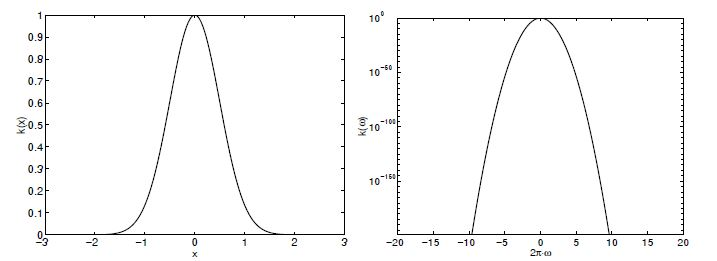
\includegraphics[width=6in]{images/Chap3_Gaussian_kernel}
	\caption{Gaussian kernel with $\epsilon = 0.125$ and its Fourier transform \cite{schsmo01}.}
	\label{fig:gaussian_kernel}
\end{figure}

Steinwart et al. in \cite{stehussco06} tries to answer questions like - which functions are contained in the RKHS induced by the Gaussian kernel, how the corresponding norms can be computed, and how the RKHS of different widths correlate to each other. 
In particular, RKHS of Gaussian kernels always have countable orthonormal bases. Theorem 3 of the paper gives the orthonormal basis functions for $\clH$ defined by the Gaussian kernel $\Kern_\epsilon$. It states that for $\epsilon >0$ and $n \in \mathbb{N}_0 := \mathbb{N} \cup \{0\}$, the sequence of functions $\{\phi_n : \Re \to \Re\}$ defined by,
\begin{equation}
\phi_n(x) := \sqrt{\frac{1}{(2\epsilon)^n n!}}x^n \exp(-x^2/4\epsilon).
\end{equation}
is an orthonormal basis for $\clH$.

Minh in \cite{min10} gives several properties of the RKHS induced by Gaussian kernels. Theorem 1 of the paper states that the RKHS $\clH$ induced by the standard Gaussian kernel is infinite dimensional, i.e. dim($\clH$) = $\infty$ and 
\begin{equation}
\clH := \Bigl\{ f = \exp(-x^2/4\epsilon) \sum_{n=0}^\infty w_n x^n: \|f\|^2_\clH = \sum_{k=0}^\infty (2\epsilon)^k k! \sum_{n=0}^k w_n^2 <\infty \Bigr\}
\end{equation}
Some of the salient properties of the Gaussian kernel RKHS are summarized below: 
\begin{arabnum}
	\item $\clH$ induced by the standard Gaussian kernel does not contain any polynomial on $\state$, including the non-zero constant function. 
	
	\item If $\state$ is compact, $\clH$ induced by the Gaussian kernel is dense in the space of $\mathcal{C}(\state)$ of continuous functions on $\state$.
	This means that given a continuous function $h(x)$, for all $\varepsilon >0$, we can find a function $g(x) \in \clH$ such that 
	\begin{equation}
	\|h(x) - g(x)\|_\infty \leq \epsilon \qquad \forall x \in \state
	\end{equation} 
	\item Let $\Kern_{\epsilon}(x,x') = \exp(-\frac{\|x-x'\|^2}{4\epsilon})$. The Hilbert space $\clH_\epsilon$ induced by $\Kern_\epsilon$ on $\state$ contains the function $\exp(-\frac{c \|x\|^2} {4 \epsilon})$ if and only if $0<c <2$. For example, $\exp(-\frac{\|x\|^2}{2 \epsilon}) \in \clH_{\epsilon/2}$, but  $\exp(-\frac{\|x\|^2}{2 \epsilon}) \notin \clH_{\epsilon}$. As $c=0$ is excluded, it validates the first property that constant functions do not belong to $\clH$.
	
	\item The functions in $\clH$ that are smooth are not necessarily integrable, as $\clH \notin L^1(\Re^n)$ for any $\epsilon >0$.  This implies that $L^1$ norm optimization or regularization is infeasible in $\clH$. This could still be done on subsets of finite linear combinations of the basis functions.
	
	
	\item Partial derivatives of the Gaussian kernel denoted as $\frac{\partial^n}{\partial x^n} \Kern_x \in \clH$. As a corollary, it can be shown that $t^n \Kern_x(t)\in\clH$. Additionally, for any polynomial $p(t)$, $p(t) \Kern_x(t) \in \clH$. An expression for the Hilbert space norm for kernel derivative of any order $d$ is also provided in \cite{min10}. 
\end{arabnum}

The paper by Michelli et al. \cite{micchaxuzha06} sets out to identify kernels with universal approximating property, i.e. given any compact set $\state$, any function $f \in \mathcal{C}(\state)$, there is a function $g \in \clH$ such that $\| f - g\|_{\infty} \leq \varepsilon$ holds for any $\varepsilon > 0$. Thus for any choice of compact set $\state$, the space $\clH$ is dense in $\mathcal{C}(\state)$ in the maximum norm. A kernel that satisfies this property is called the universal kernel. The paper discusses the characterization of universal kernels in terms of feature map representation of the kernel $\Kern$. It provides necessary and sufficient condition for $\Kern$ to have the universal approximation property in terms of its features. Under conditions provided in Theorem 17 of the paper, the standard Gaussian kernel is shown to be universal. 
